\documentclass{article}

\usepackage{tikz}
\usetikzlibrary{graphs,positioning,arrows}
\usetikzlibrary{shapes,arrows.meta}

\tikzstyle{box} = [rectangle, text centered, minimum size=6mm,
    draw=black,
    top color=white, 
    bottom color=red!50!black!20]
\tikzstyle{rounded} = [rectangle,minimum size=6mm,rounded corners=3mm, text centered, draw=black!50,top color=white,bottom color=black!20]
\tikzstyle{arrow} = [-{Latex[scale=1.2]},rounded corners]
\tikzstyle{start} = [circle,inner sep=2pt,minimum size=2pt,fill=white,draw=black!50 ]
\tikzstyle{end} = [start]

\begin{document}
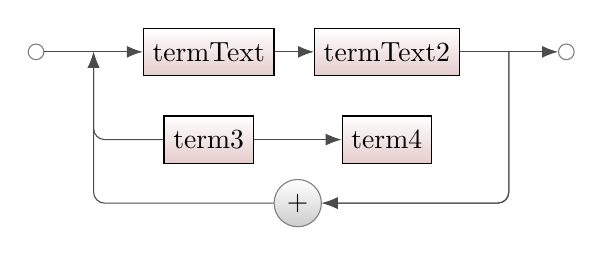
\begin{tikzpicture}[%
node distance=5mm,
%>=stealth',
black!70,
text=black,
%graphs/every graph/.style={},
%skip loop/.style={to path={-- ++(0,#1) -| (\tikztotarget)}},
%hv path/.style={to path={ -| (\tikztotarget)}},
%vh path/.style={to path={-- ++(-0.20,0.0) |- (\tikztotarget)}},
%start/.style={%
%    circle,inner sep=2pt,minimum size=2pt,fill=white,draw=black!50,
%},
%end/.style={%
%    start,
%},
]

\node[start] (start) {};
\node[right=of start] (p1) {};
\node[box,right=of p1] (term) {termText};
\node[box,right=of term] (term2) {termText2};
\node[box,below=of term] (term3) {term3};
\node[box,below=of term2] (term4) {term4};
\draw [arrow] (term) -- (term2);
\draw [arrow] (term3) -- coordinate[midway](m3)(term4);
\node[rounded,below=of m3] (plus)  {+};
\node[right=of term2] (p2) {};
\node[end,right=of p2] (end) {};


\draw [arrow] (start) -- coordinate[midway](m1)(term);
\draw [arrow] (term2) -- coordinate[midway](m2)(end);
%\draw [arrow] (plus) -- (term);
\draw [arrow] (plus) -| (m1);
\draw [arrow] (term3) -| (m1);
\draw [arrow] (m2) |- (plus);
\draw [arrow] (m2) |- (plus);

\end{tikzpicture}
\end{document}
